\documentclass[runningheads,a4paper,twoside]{llncs}
\usepackage[plmath,MeX]{polski}
\usepackage[utf8]{inputenc}
\usepackage{bookman}
\usepackage[T1]{fontenc}
\usepackage{amssymb}  % must be loaded before babel[polish]
\usepackage[polish]{babel}
\usepackage{csquotes}
\setcounter{tocdepth}{3}

\renewcommand{\subparagraph}{}  % titlesec did not work without this
                                % definition and I~don't use
                                % subparagraphs anyway.
\usepackage{titlesec}
\titlelabel{\thetitle.\quad}
\usepackage{caption}
\captionsetup[algorithm]{labelfont=rm,labelsep=colon}

\DeclareQuoteStyle{polish}
	{\quotedblbase}{\textquotedblright}
	{\quotesinglbase}{\textquoteright}

\usepackage[backend=bibtex,sorting=nyt,style=numeric-comp]{biblatex}
\DeclareLanguageMapping{polish}{src/polish}
\addbibresource{../src/bib.bib} % bibtex is run from inside of build/ directory

\let\emptyset\varnothing

\usepackage{hyperref}
\usepackage{url}
\usepackage{breakurl}

\usepackage{wrapfig}
\usepackage{graphicx}
\usepackage{epstopdf}
\usepackage[subrefformat=parens,labelformat=parens]{subfig}

\usepackage{units}

\usepackage{color}
\definecolor{gray}{rgb}{0.5,0.5,0.5}

\usepackage{listings}
\usepackage{listingsutf8}
\usepackage{chngcntr}
\lstset{
  language=C,
  basicstyle=\small,
  numbers=left,
  numberstyle=\tiny\color{gray},
  stepnumber=1,
  numbersep=5pt,
  showspaces=false,
  showstringspaces=false,
  showtabs=false,
  tabsize=8,
  captionpos=b,
  breaklines=true,
  breakautoindent,
  columns=fixed,
  escapeinside={(*}{*)},
  morekeywords={inline,bool}
}
\renewcommand*\lstlistingname{Wydruk}
\renewcommand*\lstlistlistingname{Spis wydruków}
\def\code{\lstinline[basicstyle=\itshape]}

\usepackage{algorithm}
\makeatletter
\renewcommand*{\ALG@name}{Algorytm}
\makeatother

\usepackage[noend]{algpseudocode}
\renewcommand*{\algorithmicrequire}{\textbf{Wymaga:}}
\renewcommand*{\algorithmicensure}{\textbf{Zapewnia:}}
\renewcommand*{\algorithmiccomment}[1]{{\footnotesize \itshape \{ #1 \}}}
\renewcommand*{\algorithmicif}{\textbf{Jeżeli}}
\renewcommand*{\algorithmicthen}{}
\renewcommand*{\algorithmicelse}{\textbf{wpp.}}
\renewcommand*{\algorithmicfor}{\textbf{Dla}}
\renewcommand*{\algorithmicforall}{\textbf{Dla wszystkich}}
\renewcommand*{\algorithmicdo}{\textbf{}}
\renewcommand*{\algorithmicwhile}{\textbf{Dopóki}}
\renewcommand*{\algorithmicloop}{\textbf{Wykonuj}}
\renewcommand*{\algorithmicrepeat}{\textbf{Wykonuj}}
\renewcommand*{\algorithmicreturn}{\textbf{zwróć}}
\renewcommand*{\algorithmicuntil}{\textbf{aż}}
\renewcommand*{\algorithmicfunction}{\textbf{Funkcja}}
\renewcommand*{\algorithmicprocedure}{\textbf{Procedura}}

\clubpenalty=10000
\widowpenalty=10000
\brokenpenalty=10000
\sloppy

\newcommand*{\ang}[1]{ang.\ \textit{#1}}
\newcommand{\keywords}[1]{\par\addvspace\baselineskip
\noindent\textbf{Słowa kluczowe:}\enspace\ignorespaces#1}

\title{Alokacja ciągłych fizycznie obszarów pamięci w~systemie Linux}
\author{Michał Nazarewicz}
\date{\today}
\institute{Instytut Informatyki Politechniki Warszawskiej,\\
\href{mailto:mina86@mina86.com}{\path|mina86@mina86.com|}}

\addtolength{\textheight}{1cm}

\begin{document}

\counterwithout{lstlisting}{chapter}

\mainmatter

\maketitle

\begin{abstract}
Praca opisuje problemy w~alolkacji ciągłych fizycznie obszarów pamięci
w~systemach opartych o~jądro Linux, szczególnie widoczne w~tak
zwanych systemach wbudowanych (np.\ telefonach komórkowych
i~tabletach), gdzie jednostka translacji adresów może być niedostępna
dla wielu podzespołów takich jak aparat fotograficzny, czy dekoder
wideo.

Praca przedstawia również często stosowane rozwiązania tych problemów
wykazując kłopoty z~nich wynikające, aby na koniec zaprezentować
proponowane przeze mnie rozwiązanie w~postaci alokator pamięci ciągłej
\ang{Contiguous Memory Allocator} (CMA), który pozwala przydzielać
duże ciągłe fizycznie bufory, bez konieczności rezerwowania na
wyłączność dużych obszarów przy starcie systemu.

\keywords{pamięć ciągła fizycznie, Linux, zarządzanie pamięcią}
\end{abstract}

\section{Opis problemu}

W~celu zwiększenia efektywności działania oraz liczby udostępnianych
funkcji, komputery a w~szczególności telefony komórkowe posiadają
wiele wyspecjalizowanych podzespołów.  W~wielu przypadkach, procesor
komunikuje się z~nimi poprzez bufory w pamięci operacyjnej,
przekazując do urządzenia jedynie adresy gdzie dane się znajdują.
Dostęp do RAM-u poprzez takie podzespoły może się jednak wiązać
z~wieloma ograniczeniami.

\begin{figure}[tbp]
  \centering
  \subfloat[System z~układem MMU pomiędzy procesorem a~pamięcią oraz
    urządzeniami podłączonymi bezpośrednie do szyny pamięci.]{
    \label{fig:sys-with-mmu}
    \includegraphics[width=.25\textwidth]{build/mmu-iommu-images--img-nommu.eps}
  } \qquad
  \subfloat[Systemu z~kontrolerem DMA, który pośredniczy w~transferach
    danych pomiędzy pamięcią i~urządzeniami.]{
    \label{fig:sys-with-dma}
    \includegraphics[width=.25\textwidth]{build/mmu-iommu-images--img-dma.eps}
  }\qquad
  \subfloat[Systemu z~zarówno układem MMU jak i~IOMMU, które tłumaczą
    adresy widziane przez odpowiednio procesor oraz urządzenia.]{
    \label{fig:sys-with-iommu}
    \includegraphics[width=.25\textwidth]{build/mmu-iommu-images--img-iommu.eps}
  }
  \caption[Różne przestrzenie adresowe dostępne
    w~komputerze.]{Reprezentacja systemów z~różnymi podzespołami
    uczestniczącymi w~translacji adresów lub transferach danych do
    pamięci operacyjnej.}
  \label{fig:mmu-iommu}
\end{figure}

Nowoczesne architektury przeznaczone do serwerów i~komputerów
osobistych posiadają jednostkę zarządzania pamięcią (\ang{memory
  management unit}, MMU), która tłumaczy adresy logiczne na fizyczne.
Dzięki temu, bufory ciągłe z~punktu widzenia procesora, mogą
w~rzeczywistości być podzielone na wiele części rozrzuconych po
pamięci fizycznej.  W~ten sposób, nawet jeżeli program alokuje
wielomegabajtowy obszar, system może zrealizować żądanie alokując
czterokibibajtowe strony i~nie przejmować się fragmentacją pamięci.

Niemniej, jak to przedstawia rysunek \subref*{fig:sys-with-mmu},
jednostka MMU nie jest zazwyczaj dostępny dla pozostałych układów
znajdujących się w~urządzeniu, takich jak karta dźwiękowa, czy
kontroler sieciowy.  Także i~dla tych przypadków istnieje rozwiązanie
w~postaci mechanizmu bezpośredniego dostępu do pamięci (\ang{Direct
  Memory Access}, DMA), którego celem jest odciążenie procesora od
przesyłania danych.  Co prawda urządzenie nadal znajduje się
w~przestrzeni adresów fizycznych, co ilustruje rysunek
\subref*{fig:sys-with-dma}, ale dzięki układowi DMA nieciągłość
buforów może zostać przed nim ukryta.

Niestety mechanizm bezpośredniego dostępu do pomięci jest ograniczony
do transferów sekwencyjnych.  Sprawdza się bardzo dobrze dla operacji
dyskowych, ale nie nadaje się dla sprzętowego dekodera wideo, który
potrzebuje dostępu do wielu dekodowanych ramek
jednocześnie.\footnote{Jednym z~rodzajów ramek stosowanych do
  kodowania klatki ze strumienia wideo jest b-ramka, która już nawet
  w~starszych standardach takich jak MPEG-2 może odwoływać się do
  jednej poprzedzającej i~jednej następującej klatki, a w~przypadku
  nowszego standardu H.264, może zależeć od więcej niż dwóch innych
  ramek.}

Oczywiście nie ma żadnych technologicznych przeszkód do zastosowania
jednostki translacji adresów również dla podzespołów innych niż
procesor, tak jak to przedstawia rysunek \subref*{fig:sys-with-iommu}.
Istotnie istnieją platformy sprzętowe z~MMU wejścia/wyjścia
(ang.\ IOMMU), który pozwala na budowanie dużych buforów złożonych ze
stosunkowo małych stron.  W~takich systemach, w~zasadzie nie ma (lub
nie powinno być) konieczności alokowania wielomegabajtowych ciągłych
obszarów pamięci.

Niestety, nawet jeżeli IOMMU jest dostępne na danej platformie, jego
obecność może się wiązać z~dodatkowym kosztem wynikającym
z~nieoptymalnego kodu \autocite{bib:price-of-safety} lub konieczności
odczytywania mapowań z~pamięci
\autocite{bib:mitigate-iotlb-bottleneck}.  Z~tego względu architekt
platformy może zdecydować, aby wyłączyć IOMMU i~rozwiązać problem
„w~oprogramowaniu”.

Z~uwagi na koszty i~ograniczenia zarówno kontrolerów DMA jak i~układów
MMU, w~wielu systemach wbudowanych, takich jak np.\ telefony
komórkowe, takie mechanizmy są często niedostępne.  Jednocześnie,
właśnie takie urządzenia posiadają dużo wyspecjalizowanych
podzespołów, jak chociażby aparat fotograficzny, czy układ do
dekodowania obrazów JPEG.

Powoduje to, że tego typu układy muszą operować bezpośrednio na
adresach fizycznych i~w~konsekwencji, wszelkie stosowane przez nie
bufory muszą być ciągłe.  Niestety Linux nie jest dobrze przystosowany
do alokowania takich obszarów.\footnote{W~szczególności, Linux nie
  jest nawet w~stanie (bez modyfikowania źródła) zarządzać obszarami
  większymi niż cztery mebibajty (1024 strony), gdy tymczasem
  pięciomegapikselowa kamera potrzebuje buforu o~rozmiarze 15
  megabajtów, a~pojedyncza ramka \textit{full HD} (tj.\ 1920 $\times$
  1080) zajmuje ponad sześć megabajtów.}


\section{Możliwe rozwiązania}

Ponieważ problem jest znany od dawna, na przestrzeni lat powstało
wiele rozwiązań programowych umożliwiających obejście trudność
w~alokacji dużych obszarów.  W~tym podrozdziale opiszę je pokrótce
oraz przedstawie ich ograniczenia.

\subsection{Przypisywanie pamięci na stałe}

Najprostszym, i~stosunkowo często stosowanym, rozwiązaniem jest
rezerwacja przy starcie systemu pewnego regionu pamięci na potrzeby
konkretnych sterowników.

Najłatwiejszym, acz niezbyt eleganckim sposobem jest wykorzystanie
argumentu \code|mem| jądra.  Przekazany przez program startujący
powoduje, że Linux nie stara się automatycznie wykryć dostępnej
pamięci RAM i~zamiast tego interpretuje przekazane informacje.  W~ten
sposób, możliwe jest ograniczenie widzianej przez system pamięci, tak
że ukryte regiony mogą być wykorzystywane przez konkretne sterowniki.

Bardziej eleganckim rozwiązaniem jest skorzystanie z~alokatora
memblock, który jest aktywny zanim jądro zainicjuje wszystkie swoje
podsystemy.  Jego zadaniem jest śledzenie wolnej pamięci zanim
bardziej zaawansowany alokator stron będzie dostępny w~systemie.
Wołany dostatecznie wcześnie, jest w~stanie zaalokowanie duże obszary
pamięci, które potem można wykorzystać w~dowolny sposób.

Niestety, o~ile tego typu rozwiązania mogą być wystarczające, jeżeli
podzespoły wymagają stosunkowo małych buforów, przestają się skalować
przy współczesnych systemach, gdyż wymagają rezerwacji wielu
megabajtów, które przez większość czasu nie są do niczego
wykorzystywane.

\subsection{Pula pamięci fizycznej}

Bardziej skomplikowanym rozwiązaniem jest mechanizm, który rezerwuje
pewną przestrzeń pamięci, ale zamiast na stałe przypisywać obszary do
urządzeń, pozwala sterownikom alokować bufory wtedy, gdy są one
potrzebne.

W~trakcie moich prac stworzyłem \textit{Physical Memory Manager} (PMM)
\autocite{patch:pmm}, który implementuje dokładnie te założenia. W~tym
podstawowym zastosowaniu, PMM nie przedstawia sobą nic nowego.  Już
bowiem w~1996 roku Matt Welsh napisał pierwszą wersję patcha
\emph{bigphysarea} dla jądra 1.3.71, który był z~różnym zaangażowaniem
utrzymywany i~przystosowywany aż do wersji 3.2 Linuksa
\autocite{patch:bigphys}.

PMM umożliwiał jednak alokowanie dużych obszarów ciągłej pamięci
fizycznej nie tylko sterownikom działającym w~przestrzeni jądra, ale
także programom działającym pod kontrolą systemu. Co więcej, dzięki
integracji z~mechanizmem współdzielenia pamięci Systemu
V~(tj.\ funkcjami \code|shmget|, \code|shmat|, \code|shmdt| itp.)
wykorzystywanym między innymi przez X~Window, PMM pozwalał na
dekodowanie obrazów i~strumieni wideo bezpośrednio do buforów
dostępnych dla serwera X11.  Dzięki temu, w~całym procesie dane nie
były niepotrzebnie kopiowane, co minimalizowało użycie procesora
i~szyny pamięci przyśpieszając działanie systemu.

Jednakże, pamięć zarezerwowana przez PMM i~tak przez większość czasu
była zupełnie nieużywana, a~więc marnowana.  Z~tego powodu, PMM nie
został przyjęty przez społeczność programistów Linuksa i~musiałem
rozwijać inne rozwiązanie.

\subsection{Zarys Contiguous Memory Allocatora}

W~ten sposób zrodził się alokator pamięci ciągłej, \textit{Contiguous
  Memory Allocator} (CMA), który umożliwia systemowi używanie
zarezerwowanej pamięci, o~ile żadne urządzenie jej w~danym momencie
nie potrzebuje.

Pierwsze wersje alokatora CMA skupiały się w~dużej mierze na
umożliwianiu sterownikom alokowania różnych buforów w~różnych
obszarach pamięci.  Było to potrzebne, gdyż dekoder wideo stosowany na
platformie S5PV110 wymagał, aby różne dane były przechowywane
w~różnych bankach pamięci.  Pozwalało to na zwiększenie szybkości
dostępu do tych danych dzięki zastosowaniu odczytu z~dwóch banków
pamięci jednocześnie.

Z~czasem, coraz bardziej integrowałem mechanizm CMA z~kodem
zarządzania pamięci w~Linuksie w~wyniku czego, pamięć rezerwowana przy
starcie, stała się dostępna dla reszty systemu, o~ile żaden sterownik
jej nie używał \autocite{patch:cma-24}.  Takie rozwiązanie zostało
ostatecznie zaakceptowane przez społeczność deweloperów Linuksa i~jest
dostępne począwszy od wersji 3.5 jądra.

\chapter{Zapoznanie z~alokatorem stron}

Ponieważ CMA integruje się dość mocno z~podsystemem zarządzania
pamięci (\ang{memory management}), do jej zrozumienia potrzeba
choć ogólnej wiedzy na temat tego w~jaki sposób Linuks zarządza
pamięcią \TODO{powtórzenie zarządza pamięcią}.

Linuks posiada wiele mechanizmów dzięki którym sterowniki mogą
alokować pamięć.  Począwszy od funkcji \lstinline|kmalloc()|
i \lstinline|vmalloc()|, poprzez mechanizmy puli pamięci, aż do
alokatora czasu bootowania i~alokatorów pamięci dostępnej dla urządzeń
zewnętrznych \cite[rozdział 8]{bib:ldd3}.  Pomimo, tak dużej liczby
interfejsów, wiele z~nich sprowadza się do alokatora stron (\ang{page
  allocator}), który jest sercem całego podsystemu zarządzania
pamięcią.

\section{Algorytm bliźniaków}

\begin{wrapfigure}{o}[1.5cm]{0.3\textwidth}
\begin{center}
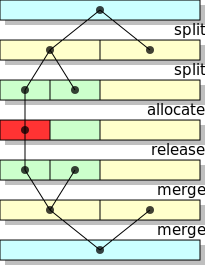
\includegraphics[width=0.25\textwidth]{build/alloc-free-cycle.eps}
\end{center}
\caption{Graficzna reprezentacja cyklu alokacji i~zwalniania buforów
  w~algorytmie bliźniaków.}
\end{wrapfigure}

Alokator stron implementuje algorytm bliźniaków (skąd też jego inna
angielska nazwa: {\it buddy system} lub {\it buddy allocator}), który
operuje na blakach o~rozmiarze $2^k$ jednostek.  W~przypadku Linuksa
jednostką jest pojedyncza strona fizyczna, a~na $k$~narzucone jest
ograniczenie $k < \mathrm{MAX\_ORDER}$.  \lstinline|MAX_ORDER| może
zależeć od architektury, na którą Linuks jest kompilowany, ale
zazwyczaj ma wartość $11$ (toteż na potrzeby tej pracy zakładam, iż $0
\le k \le 10$).

W~Linuksie, przez $k$ rozumie się rząd\TODO{może po prostu lepiej
  zostawić „order” i~nie tłumaczyć?} strony (\ang{page order}).
Strona rzędu 0 to pojedyncza strona fizyczna, strona rzędu 1
(\ang{1-order page}) to dwie strony fizyczne itd.\ aż do strony rzędu
10, czy też strony maksymalnego rzędu (\ang{max order page}), która
składa się z~1024 stron fizycznych.  Ogólnie, strona rzędu $n$ składa
się z~dwóch stron rzędu $n-1$.

Funkcja \lstinline|alloc_pages()|, która jest interfejsem dla
alokatora stron, przyjmuje jako argument właśnie rząd żądanej strony.

Z~powyższego opisu wynikają następujące właściwości alokatora stron.

\begin{itemize}
\item Nie można za jego pomocą zaalokować mniej niż jednej strony,
  tj.\ 4096 bajtów.
\item Interfejs zwyczajnie nie pozwala alokować obszarów, których
  rozmiar nie jest potęgą dwójki.
\item Gdyby jednak chcieć zaalokować taki obszar, wiązałoby się to
  z~potencjalnie dużą fragmentacją wewnętrzną.  Dla przykładu bufor
  dla kolorowej tekstury o~rozmiarze $512 \times 512$ pikseli
  wymagałby obszaru o~rozmiarze \unit[1]{MiB}, z~których
  \unit[256]{KiB}, a~więc \nicefrac{1}{4}, byłoby nieużywane.
\item Alokator stron nie jest w~stanie zaalokować obszaru większego
  niż \unit[4]{MiB}.  Z~tego powodu, nie nadaje się do alokowania
  ciągłego fizycznie buforu dla 5 megapikselowej kamery, czy nawet dla
  pojedynczej ramki {\it full HD}.
\end{itemize}

Jak zatem działa algorytm bliźniaków?  Alokator posiada listę wolnych
stron, których rząd jest pomiędzy $0$ a~$10$.  W~Linuksie zrealizowane
jest to poprzez 11 list dwukierunkowych, gdzie każda przeznaczona jest
dla stron o~konkretnym rzędzie.

Gdy sterownik chce zaalokować stronę rzędu $n$, alokator sprawdza
odpowiednią listę.  Jeżeli jest ona pusta, przechodzi do listy ze
stronami rzędu $n+1$, aż znajdzie wolną stronę (lub dojdzie do
maksymalnego rzędu, co sygnalizuje nieudaną alokację.  Jeżeli uzyskana
w~ten sposób strona ma rząd większy niż żądany, jest ona dzielona na
pół, aż do osiągnięcia żądanego rozmiaru.  Strony, które powstały na
skutek podziału większej strony na pół, nazywamy stronami
bliźniaczymi.  Cały proces ilustruje algorytm \ref{alg:buddy-alloc}

\begin{algorithm}\label{alg:buddy-alloc}
\caption{Alokacja strony rzędu $k$ w~algorytmie bliźniaków}
\begin{algorithmic}[1]
\Require $0 \leq k < \mathrm{MAX\_ORDER}$
\Function{AllocatePage}{$k$}
    \State $i \gets k$
    \While {lista stron rzędu $i = \emptyset$}
        \State $i \gets i + 1$
        \If {$i = \mathrm{MAX\_ORDER}$}
            \State \Return $\emptyset$
        \EndIf
    \EndWhile

    \State $p \gets$ strona z listy stron rzędu $i$
    \While {$i \neq k$}
        \State $i \gets i - 1$
        \State podziel $p$ na pół na $p_1$ i $p_2$
        \Comment{Strony $p_1$ i $p_2$ nazywamy stronami bliźniaczymi}
        \State $p \gets p_1$
        \State dodaj $p_2$ do listy stron rzędu $i$
    \EndWhile
    \State \Return $p$
\EndFunction
\end{algorithmic}
\end{algorithm}

Przy zwalnianiu, dopóki to możliwe, strona jest łączona ze swoją
bliźniaczą stroną, dzięki czemu strony są dodawane do listy wolnych
stron o~dużym rzędzie.  Proces ten ilustruje algorytm
\ref{alg:buddy-free}

\begin{algorithm}\label{alg:buddy-free}
\caption{Zwalnianie strony $p$ rzędu $k$ w algorytmie bliźniaków}
\begin{algorithmic}[1]
\Procedure{FreePage}{$p$, $k$}
    \While {$k + 1 \neq \mathrm{MAX\_ORDER} \wedge p$ posiada wolną stronę bliźniaczą}
        \State $p' \gets$ strona bliźniacza $p$
        \State usuń $p'$ z~listy wolnych stron
        \State $k \gets k + 1$
        \State $p~\gets$ strona powstała w~wyniku połączenia $p$ i~$p'$ \label{alg:buddy-free:join}
    \EndWhile
    \State dodaj $p$ do listy wolnych stron rzędu $k$\label{alg:buddy-free:add}
\EndProcedure
\end{algorithmic}
\end{algorithm}


\section{Typy migracji}\label{sec:migratetype}

Powyższy opis pomija niektóre szczegóły alokatora stron.  Po pierwsze,
nawet jeżeli w~danej chwili nie istnieje wolna strona o~żądanym
rzędzie, aktywowana jest tzw.\ wolna ścieżka (\ang{slow path}), która
wykorzystuje różne mechanizmy odzyskiwania pamięci (np.\ poprzez
zwalnianie buforów dyskowych, czy w~najgorszym przypadku zabiciu
jednego z~działających procesów).  Mechanizmy te nie są jednak istotne
dla tematyki niniejszej pracy i~dlatego zostały pominięte.

Ważnym czynnikiem są typy migracji (\ang{migratetype}), których jest
sześć: {\it unmovable}, {\it reclaimable}, {\it movable}, {\it cma},
{\it reserve} oraz {\it isolate}).

\begin{itemize}
\item Dla potrzeb tej pracy traktuję typy {\it unmovable}, {\it
  reclaimable} i~{\it reserve} jak jeden typ -- typ nieruchomy.  To
  uproszczenie wynika z~faktu, iż dla CMA-y istotne jest tylko
  rozróżnienie pomiędzy stroną ruchomą i~nieruchomą.
\item Strony które są typu ruchomego charakteryzują się tym, że ich
  adres fizyczny nie jest istotny, w~związku z~czym mogą być
  przeniesione w~inne miejsce pamięci RAM.
\item Typ cma jest nowym typem dodanym przez CMA i~jest opisany
  dokładniej w~podrozdziale \ref{sec:migrate-cma}
\item Typ {\it isolate} jest niejako pseudo-typem, gdyż jeżeli wolna
  strona ma taki typ, nie może ona zostać zaalokowana.  Więcej na
  temat sposobu w~jaki ten typ może być wykorzystywany opisuję
  w~podrozdziale \ref{sec:alloc-contig-range}
\end{itemize}

Jednym z~przykładów stron ruchomych są strony anonimowe działających
procesów.  Ponieważ program odwołują się do nich poprzez mapowania
wirtualne, o~ile tablice translacji zostaną uaktualnione, zawartość
strony może być przeniesiona w~dowolne miejsce.  Podobnie wygląda
sprawa z~buforami dyskowymi i~wieloma innymi strukturami, którymi
zarządza jądro.

Proces przenoszenia ruchomej strony z~jednego miejsca w~inne nazywa
się migracją i wykorzystywany jest między innymi przy obsłudze
hot-swapu pamięci, a~także w~trackie procesu zagęszczania (opisanego
w~\cite{bib:compaction}), którego celem jest zwiększenie liczby
dostępnych stron o~wysokich rzędach.

Wołając funkcję \lstinline|alloc_pages()|, typ migracji strony jest
przekazywany jako argument, co pozwala alokatorowi stron grupować
strony tego samego typu.  Jest to istotne, gdyż mechanizm zagęszczania
nie działa zbyt dobrze jeżeli ruchome strony przelatają się
z~pozostałymi stronami, które nie podlegają migracji.

\section{Grupy stron}

Grupowanie to realizowane jest poprzez podział pamięci na bloki
składające się z~\lstinline|pageblock_nr_pages| stron (czy też
równoważnie na bloki rzędu \lstinline|pageblock_order|).  Konkretne
wartości tych stałych zależą od architektury, no którą jądro zostało
skompilowane, jak i~opcji konfiguracyjnych wybranych w~trakcie
kompilacji.  Niemniej, przeważnie wartość tych stałych to odpowiednio
1024 (stron) i~(rząd) 10 i~właśnie takie są przyjęte w~tej pracy.

\begin{figure}[tbh]
\begin{center}
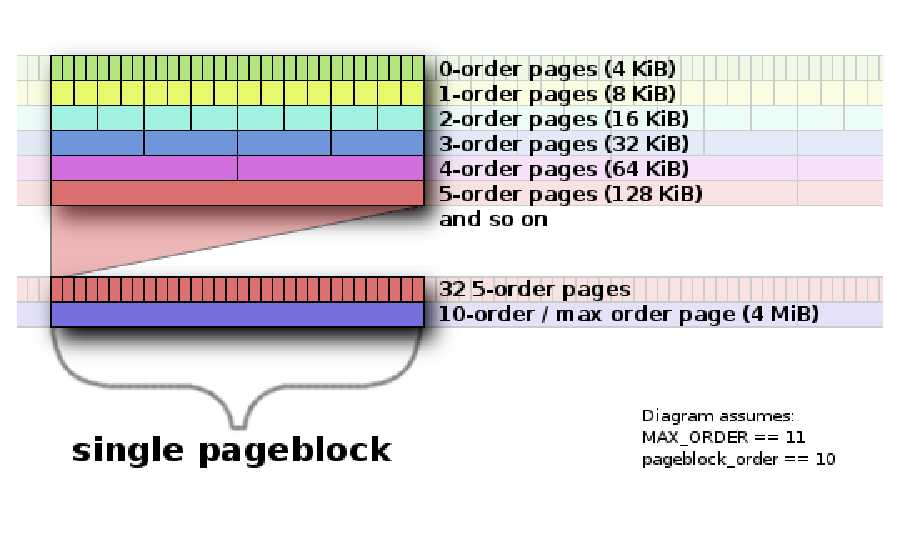
\includegraphics[width=0.8\textwidth]{build/pages.eps}
\end{center}
\TODO{przetłumaczyć, przerobić na SVG}
\caption{Graficzna reprezentacja organizacji stron pamięci stosowanej
  przez Linuksa.}
\end{figure}

Każdy blok stron (\ang{pageblock}) ma przypisany typ migracji,
a~alokator stron posiada oddzielne listy wolnych stron dla każdego
typu migracji.  Zatem patrząc na algorytm \ref{alg:buddy-alloc} należy
zdawać sobie sprawę, iż rozpatruje on listy wolnych stron danego typu
migracji.

\section{Zmiana typu migracji}\label{sec:type-change}

Należy pamiętać, iż dla jądra zrealizowanie alokacji jest ważniejsze
od trzymania stron o~tym samym typie migracji razem.  Dlatego dla
każdego typu migracji istnieje lista zapasowych (\ang{fallback}) typów
migracji.  Jeżeli alokacja dla żądanego typu migracji nie powiedzie
się, alokator stron będzie próbował z~kolejnymi typami z~list, tak jak
to pokazuje algorytm \ref{alg:buddy-fallback}

Co więcej, jeżeli rząd żądanej strony jest dostatecznie duży, typ
migracji wszystkich wolnych stron w~danym bloku zostaje zmieniano na
ten zgodny z~wywołaniem funkcji \lstinline|alloc_pages()|.

\begin{algorithm}\label{alg:buddy-fallback}
\caption{Alokacja strony rzędu $k$ z~uwzględnieniem typu migracji $m$}
\begin{algorithmic}[1]
\Function{ChangeBlockMigrateType}{$b$, $m$}
\State zmień typ migracji $b$ na $m$
\ForAll {wolnych stron $p' \in b$}
    \State przenieś $p'$ na listę wolnych stron typu $m$
\EndFor
\EndFunction
\Statex
\Function{AllocPageMigrateType}{$k$, $m$}
    \State $f \gets$ lista zapasowych typów migracji dla typu $m$
    \State dodaj $m$ na początek $f$
    \ForAll{$m' \in f$}
        \State $p \gets$ \Call{AllocPage}{$k$} biorąc pod uwagę listy stron typu $m'$
        \If {$p \neq \emptyset$}
            \If {$m \neq m' \wedge k \geq \nicefrac{\mathrm{page\_order}}{2}$}
                \State $b \gets$ blok stron zawierający $p$
                \State \Call{ChangeBlockMigrateType}{$b$, $m$}
            \EndIf
            \State \Return $p$
        \EndIf
    \EndFor
    \State \Return $\emptyset$
\EndFunction
\end{algorithmic}
\end{algorithm}

Podczas zwalniania, gdy strona jest dodawana do listy wolnych stron
(wideczne w~linii \ref{alg:buddy-free:add} algorytmu
\ref{alg:buddy-free}) typ migracji listy, na którą strona trafia
determinowany jest poprzez typ migracji przypisany blokowi stron do
którego dana strona należy.

Istotne jest tutaj, aby zauważyć, iż bloki stron mogą zmieniać swój
typ migracji, a~także, że nawet jeżeli blok ma dany typ migracji,
strony o~innym typie migracji mogą być z~niego przydzielone.


\section{Listy PCP}\label{sec:pcp-lists}

Ostatnim istotnym, z~punktu widzenia CMA, aspektem alokatora stron są
listy PCP.  Ponieważ listy wolnych stron są współdzielone w~obrębie
całego systemu dostęp do nich musi być synchronizowany pomiędzy
wszystkimi procesorami.  Aby uniknąć kosztów związanych
z~synchronizacją, każdy procesor posiada swoje prywatne PCP listy, na
których znajdują się wolne strony rzędu 0.  Biorąc również i~ten
aspekt pod uwagę, alokacja przyjmuje postać przedstawianą w~algorytmie
\ref{alg:buddy-pcp}

\begin{algorithm}\label{alg:buddy-pcp}
\caption{Alokacja strony rzędu $k$ z~typem migracji $m$
  z~uwzględnieniem list PCP}
\begin{algorithmic}[1]
\Function{AllocPageUsePCP}{$k$, $m$}
    \If {$k \neq 0$}
        \State $p \gets$ \Call{AllocPageMigrateType}{$k$, $m$}
    \Else
        \State $l \gets$ lista PCP dla typu migracji $m$
        \If {$l = \emptyset$}
            \State $i \gets 0$
            \Repeat
                \State $p \gets$ \Call{AllocPageMigrateType}{$0$, $m$}
                \If {$p \neq \emptyset$}
                    \State dodaj $p$ do $l$
                    \State $i \gets i + 1$
                \EndIf
            \Until {$i \geq n \vee p = \emptyset$} \Comment{Wartość
              $n$ jest zależna od różnych czynników}
        \EndIf
        \If {$l = \emptyset$}
            \State \Return $\emptyset$
        \Else
            \State $p \gets$ pierwsza strona z $l$
            \State usuń pierwszą stronę z $l$
            \State lista PCP dla typu migracji $m$ $\gets l$
        \EndIf
    \EndIf
    \State \Return $p$
\EndFunction
\end{algorithmic}
\end{algorithm}

\section{Implementacja i~sposób działania mechanizmu CMA}

Podstawowym założeniem alokatora CMA jest umożliwienie alokowania
dużych obszarów ciągłych fizycznie bez konieczneści rezerwacji na
wyłączność dużej ilości pamięci.  Aby to umożliwić, interfejs CMA
korzysta z~mechanizmu migracji stron opisanego pokrótce w~podrozdziale
\ref{sec:migratetype}.  Ogólny zarys alokacji z~regionów CMA
przedstawiony jest na rysunku \ref{fig:cma-alloc-algo} a~niniejszy
rozdział opisze ją w~większych szczegółach.

\begin{figure}[tbp]
  \includegraphics[width=\textwidth]{build/cma-alloc-algo.eps}
  \caption{Schemat działania alokatora CMA.}
  \label{fig:cma-alloc-algo}
\end{figure}


\subsection{Typ migracji CMA}\label{sec:migrate-cma}

Migracja jest możliwa tylko dla stron ruchomych.  Niestety, przed
zaimplementowaniem alokatora CMA, Linux nie posiadał mechanizmu, który
pozwalałby zagwarantować istnienia dużego obszaru, w~którym strony są
albo wolne, albo ruchome.  Ponieważ (jak opisałem w~podrozdziale
\ref{sec:type-change}) jądro dopuszcza alokacje nieruchomych stron
z~bloków ruchomych, a~także posiada mechanizm na skutek którego bloki
zmieniają swój typ, aby mechanizm CMA mógł działać poprawnie, należało
stworzyć nowy typ migracji -- nazwanym po prostu typem migracji cma --
który posiada dwie bardzo istotne cechy: (i) z~bloków oznaczonych
typem cma mogą być alokowane tylko strony ruchome, oraz (ii) blok
oznaczony typem cma nie zmienia swojego typu (na skutek działania
alokatora stron).

O~ile pierwsza właściwość jest stosunkowo prosta do osiągnięcia,
zagwarantowanie niezmienności typu bloku stron wymagało
zidentyfikowania wszystkich sytuacji, w~których blok może zmienić swój
typ i~dodanie odpowiednich warunków zapewniających, że niepożądana
zmiana nie nastąpi.

\subsection{Alokowanie wybranego obszaru pamięci}\label{sec:alloc-contig-range}

Posiadając gwarancję, że dany zakres składa się jedynie z wolne
i~ruchome stron, można przystąpić do jego alokacji.  Drugim krokiem
implementowania alokatora CMA było zatem stworzenie funkcji, która
dostaje jako argument zakres stron, a~następnie migruje wszystkie
zajęte strony, a~wolne usuwa z~listy wolnych stron.  Właśnie to czyni
funkcja \code|alloc_contig_range|.

Pierwszym krokiem wykonywanym przez tę funkcję jest zmiana typu bloków
stron na izolowany typ migracji.  Pomimo, że izolowane strony są
przechowywane na liście wolnych stron i~są pod kontrolą alokatora
stron, nie są one używano do zaspokajania żądań alokacji.  W~ten
sposób, funkcja \code|alloc_contig_range| uzyskuje gwarancje, że
w~trakcie jej działania strony, na których operuje nie zostaną
zaalokowane dla innych wątków jądra.

W~dalszej części wołana jest kolejna stworzona przeze mnie funkcja
\code|__alloc_contig_migrate_range|, której zadaniem jest
zidentyfikowanie i~zmigrowanie wszystkich zajętych stron z~podanego
zakresu.  Funkcja ta szukac stron, które mogą zostać zmigrowane, po
czym zleca migracje funkcji \code|migrate_pages|.

Gdy strony są już wolne i~przechowywane na liście stron izolowanych,
funkcja \code|alloc_contig_range| może usunąć je z~tej listy, na
skutek czego alokator stron zupełnie nie zdaje sobie sprawy z~ich
istnienia (co jest równoważne z~alokacją tych stron).

Aby zakończyć alokację wystarczy już przywrócić pierwotny typ bloku
(gdyż na początku został on zmieniony na typ izolowany) i~zwrócić
wskaźnik na pierwszą zaalokowaną stronę.


\subsection{Wybór zakresu stron}\label{sec:alloc-from-contig}

Alokacje CMA odbywają się z~regionów, które są rezerwowane przy
starcie systemu.  Dla każdego zarezerwowanego obszaru tworzona jest
struktura \code|cma| reprezentujące pojedynczy kontekst CMA.  Posiada
ona następujące pola:

\begin{tabular}{lll}
\textbf{\code|base_pfn|} & Identyfikator pierwszej strony w~regionie. \\
\textbf{\code|count|}    & Liczba strony w~regionie. \\
\textbf{\code|bitmap|}   & Bitmapa zajętych stron. \\
\end{tabular}

Pierwsze dwa identyfikują obszar w~pamięci fizycznej, gdzie znajduje
się kontekst CMA, a~ostatnia jest mapą określającą, które ze stron
zostały zaalokowane przez CMA.  Bitmapa jest wykorzystywana przez
funkcję \code|dma_alloc_from_contiguous|, która używa metody „pierwszy
pasujący” do wyszukania dostatecznie dużego obszaru niezaalokowanych
przez CMA stron.  Po wybraniu obszaru, wołana jest funkcja
\code|alloc_contig_range|, aby dany obszar zaalokować i~jeżeli się to
powiedzie, oznacza obszar w~bitmapie jako zajęty i~zwraca wynik.

Aby nie załączać zbyt wielu szczegółów, poprzedni podrozdział nie
opisuje sytuacji, w~których alokacja może się nie powieść, ale takie
istnieją\footnote{W~istocie, jest ich dość sporo i~obecnie wraz
  z~innymi deweloperami Linuksa staram się wyszukać i~wyeliminowaniem
  takie sytuacji.  Linux, a~szczególnie zarządzanie pamięcią
  w~Linuksie, jest jednak skomplikowany i~czasem trudno prześledzić
  wszystkie zależności i~interakcje pomiędzy komponentami, które mogą
  prowadzić do błędu alokacji.} i~z~tego powodu, funkcja
\code|dma_alloc_from_contiguous| działa w~pętli próbując alokować aż
do skutku różne obszaru.

\section{Podsumowanie}

Dołączenie CMA w~czerwcu 2012 r.\ do Linuksa w~żadnym stopniu nie
oznacza zakończenia nad nim prac.  Nadal jest wiele właściwości, które
można usprawnić i~nowych funkcji, które można dodać.

Najistotniejszym aspektem CMA jest czas potrzebny na zrealizowanie
alokacji.  Migracja tysięcy stron może być czasochłonna, gdyż nawet
w~systemach z~szybką magistralą, kopiowanie kilkudziesięciu megabajtów
danych może trochę potrwać.

\textcite{patch:cma-discard} zaimplementował we wrześniu 2012
r.\ usprawnienie, które w~istotny sposób skraca czas alokacji.
W~swoich testach zauważył przyśpieszenie alokacji \unit[10]{MiB}
z~\unit[146]{ms} do zaledwie \unit[7]{ms}.  Pomysł polega na
odrzucaniu stron które można w~prosty sposób odzyskać.  Najprostszym
przykładem są tutaj bufory dyskowe\,---\,ich zawartość można
przywrócić ponownie odczytując dane z~nośnika.

Innym możliwym usprawnieniem CMA jest ulepszenie algorytmu doboru
zakresu stron.  Obecnie stosowana metoda „pierwszy pasujący” nie
uwzględnienia, które strony wymagają migracji.  Może to powodować, iż
alokator będzie dokonywał migracji, którym można było zapobiec.  Na
chwilę obecną nie wiadomo jednak, czy zysk z~nowego algorytmu nie
zostałby przysłonięty kosztami wynikającymi z~jego złożoności jak
i~możliwą większą fragmentacją.

Innym dość uciążliwym problemem, z~którym CMA musi sobie radzić jest
fakt, że strony ruchome nie zawsze można migrować, co może być
spowodowane brakiem funkcji migrującej lub chwilowym wykorzystaniem
strony w~kontekście wymagającym stałego adresu fizycznego.

Do pierwszej kategorii należą np.\ strony wykorzystywane przez wiele
systemów plików.  Nawet w~bardzo popularnym i~powszechnie używanym
systemie plików ext4, strony dziennika nie posiadają zaimplementowanej
funkcji migracji.

Druga kategoria to sytuacje, gdy strona została unieruchomiona na
czas, gdy wykonywany jest na niej transfer DMA.  Przykładowo, jeżeli
dane są kopiowane pomiędzy taką stroną, a~dyskiem twardym.  Jednym
z~rozważanych przeze mnie rozwiązań było migrowanie strony poza region
CMA zanim zostanie ona unieruchomiona, ale niestety sytuacja taka jest
na tyle powszechna, że degradacja wydajności byłaby zbyt duża.

Innymi możliwymi rozwiązaniami jest ograniczenie wykorzystywania
regionów CMA tylko do funkcji takich jak:

\begin{itemize}
\item mechanizm zRam \autocite{patch:zram}, który umożliwia tworzenie
  kompresowanego pliku wymiany w~pamięci, oraz
\item pamięć transcendentna \autocite{bib:transcendent} i interfejs
  \code|POSIX_FADV_VOLATILE|, które dają jądru możliwość odrzucenia
  wybranych danych zwalniając tym samym dane strony pamięci.
\end{itemize}

Z~drugiej strony w~znacznym stopniu zmniejszyłoby to użyteczność stron
z~regionu CMA, potencjalnie do tego stopnia, iż przez większość czasu
nie byłyby one zupełnie wykorzystywane.

Widać, że droga przed alokatorem CMA jest otwarta i~istnieje wiele
aspektów, które można ulepszać, a~dzięki coraz większemu gronu osób
zainteresowanych tym kodem, można pokusić się o~predykcję, iż
mechanizm CMA będzie się rozwijał.  Równocześnie kolejne osoby
wykazują zainteresowanie korzystania z~niego w~systemach znacznie
różniących się od platform, dla których był projektowany
(tj.\ telefonów komórkowych), takich jak zarządcy maszyn wirtualnych
jak i~oprogramowanie samolotów.


\appendix
\printbibliography

\end{document}
